\documentclass{scrartcl}

% Adapted from an original template by Hlyni Arnórssyni, Reykjavik University, Iceland
%
% ------------------------------ SETTINGS
\usepackage{geometry}

\geometry{
	paper=a4paper, % Paper size
	top=2.5cm, % Top margin
	bottom=2.5cm, % Bottom margin
	left=2.5cm, % Left margin
	right=2.4cm, % Right margin
	headheight=0.75cm, % Header height
	footskip=1.5cm, % Space from the bottom margin to the baseline of the footer
	headsep=0.75cm, % Space from the top margin to the baseline of the header
	%showframe, % Uncomment to show how the type block is set on the page
}

\usepackage{blindtext}
%-------------------------------- Character encoding ----------------------------
\usepackage[T1]{fontenc}
\usepackage[utf8]{inputenc}

%----------------------------- Mathematics packages from AMS ---------------

\usepackage{amsmath, amsfonts, amsthm, amssymb}
\usepackage{braket, nicefrac}

% ----------- International System of Units
\usepackage{siunitx}

%------------------------------ Lists / numbers -------------------------
\usepackage{enumitem, multicol}

%------------------------------- Figure insertions --------------
\usepackage{graphicx, float}  % Use option [H] to force the placement of a figure
\usepackage{keystroke}
\usepackage{pgfplots}\usepgfplotslibrary{units}\pgfplotsset{compat=1.16}

%------------------------------- Line Spacing --------------
\usepackage{setspace}

%------------------------------- Depth of the ToC --------------
\setcounter{tocdepth}{2}

%%%%%%%%%%%%%%%%%%%%%%%%%% Hyperlink References %%%%%%%%%%%%%%%%%%%%%%%%%%%
\usepackage{hyperref}

%--------------------% Storage Path for images %-----------------%
\graphicspath{{graphics/}{Graphics/}{./}}

%%%%%%%%%%%%%%%%%%%%%%%%%% Environments %%%%%%%%%%%%%%%%%%%%%%%%%%%
\renewenvironment{abstract}{
    \begin{center}
    \textbf{Abstract}
    \vspace{0.5cm}
    \par\itshape
    \begin{minipage}{0.8\linewidth}}{\end{minipage}
    \noindent\ignorespaces
    \end{center}
}

\newenvironment{keywords}{
    \begin{center}
    \textbf{Keywords}
    \vspace{0.5cm}
    \par
    \begin{minipage}{0.8\linewidth}}{\end{minipage}
    \noindent\ignorespaces
    \end{center}
}

\newenvironment{preface}{
    \begin{center}
    \textbf{Preface}
    \vspace{0.5cm}
    \par
    \begin{minipage}{0.8\linewidth}}{\end{minipage}
    \noindent\ignorespaces
    \end{center}
}

\newenvironment{acknowledgements}{
    \begin{center}
    \textbf{Acknowledgements}
    \vspace{0.5cm}
    \par
    \begin{minipage}{0.8\linewidth}}{\end{minipage}
    \noindent\ignorespaces
    \end{center}
}
\usepackage{graphicx}
\usepackage{listings}
\usepackage{hyperref}
\usepackage{xcolor}
\lstset { %
    language=Python,
    backgroundcolor=\color{black!5}, 
    breaklines=true,
}


\begin{document}


\begin{titlepage}
	\centering
	
\includegraphics[width=0.6\textwidth]{Graphics/CU E LOGO.png}\par
	\vspace{1cm}
	{\scshape\LARGE MECE4520 \par}      
 
	\vspace{1cm}
	{\scshape\Large Final Report - Fall 2022\par}
	%{\large \today\par}
	\vfill
	
	%%%% PROJECT TITLE
	{\huge\bfseries Laptop Price Prediction\par}
	\vfill
	
	%%%% AUTHOR(S)
	{\Large Group 11 \\Xiangzhou Jian xj2266\\Xinyi Yang xy2542\\Zhanduo Xu zx2415\\Zhexuan Tan zt2314\\Zujin Wen zw2788\\}\par
	\vspace{1.5cm}

	\vfill
	{\Large Instructor: Changyao Chen}\par



	\vfill
% Bottom of the page
\end{titlepage}


\newpage



\doublespacing
\tableofcontents
\singlespacing

\newpage

\doublespacing


\section{INTRODUCTION}

After 40 years of progress since the invention of the laptop in 1984, Laptops have been utilized for numerous purposes, for example, business, education, and recreational purposes. It is no secret that living a mobile lifestyle at home and work has become the new standard for people nowadays. Users expect and need to be able to access their computers from anywhere, whether the kitchen table or the office, which calls for portable devices. While desktop PC sales are down, laptop sales are increasing and are predicted to continue. The laptop market segment was on a steadily increasing revenue trajectory even before the epidemic, growing from \$132 billion in 2018 to \$140 billion in 2020, according to a survey from Statista. \par
~\\
\noindent However, due to remote working, learning, and increasing demand for gaming, laptop sales soared dramatically throughout the pandemic in the past 3 years, the corresponding price of which also fluctuated rapidly, especially when comparing the price between online and brick-and-mortar stores, some shocking price difference may be found in the same laptop model. Because of the lack of awareness of the price change, customers keep suffering from spending too much money on products that are not worth it. To tackle this problem, the team focused on a dataset from Kaggle and managed to build models using linear regression and neural network regression \cite{chen} to predict laptop prices. 

\section{DATA COLLECTION & ANALYZE}


\subsection{DATA SELECTION & COLLECTION }
Predicting the price of the laptop market needs numerous data, especially for crossing categories prediction and recognizing relationships between vast elements. After researching the laptop components’ category and correlation, the research team selected data from Kaggle 2020 laptop price dataset \cite{kumar_2022}. Kaggle, as a reliable data source, was selected and supervised by many data science researchers, providing detailed data on various factors, including laptop components. With every significant part of the laptop, the dataset also provides lightly-important categories, including weight, RAM, and memory details, which could be used as rows of elements for analyzing more possible results. Kaggle brings a simple data format that is simple to code, supports python programming, and is easily suitable for data preprocessing and visualization. \par

~\\
\noindent The original data contains a large amount of computer hardware information, including different brands and models of the same type of hardware. The team decided to parameterize the specific computer hardware by finding objective running scores to make the hardware part of the original data set analyzable. Through the search of team members, it was unanimously determined that finding benchmarks \cite{passmark} on reliable public websites is a feasible way to parameterize different hardware in this case. 


\subsection{DATA PROCESSING}
After querying the data, the team found that the running scores of some hardware had no reference and logic, which made a small part of the hardware running scores far from the regular CPU. Through in-depth research, it is found that a minimal amount of hardware cannot extract this type of hardware from the user because the notebook computer manufacturer uses outdated products and OEM (original equipment manufacturer) products, which leads to the abnormality of this small number of parameters. After screening, the team deleted a few hardware data with abnormal running score results. It was determined that this part of abnormal data had no reference significance in this analysis.\par
~\\
\noindent The general selling price from each memory manufacturer determined the memory benchmark, which significantly provides the difference of performance and price for each memory. However, the team's research found the price and performance of memory are highly connected. Then the dataset after processing is as shown in Table~\ref{tab:Odata}.
~\\

\begin{table}[ht]
\centering
\resizebox{17cm}{!}{
\begin{tabular}{cccccccc}
\cline{1-7}
\multicolumn{1}{|c|}{Product}           & \multicolumn{1}{c|}{CPU\_Benchmark} & \multicolumn{1}{c|}{Memory\_benchmark} & \multicolumn{1}{c|}{GPU\_benchmark} & \multicolumn{1}{c|}{Weight} & \multicolumn{1}{c|}{Ram\_benchmark} & \multicolumn{1}{c|}{Price\_euros} &                      \\ \cline{1-7}
\multicolumn{1}{|c|}{Inspiron 3567}     & \multicolumn{1}{c|}{2273}           & \multicolumn{1}{c|}{39.99}             & \multicolumn{1}{c|}{1.1}            & \multicolumn{1}{c|}{1.25kg} & \multicolumn{1}{c|}{4GB}            & \multicolumn{1}{c|}{389}          &                      \\ \cline{1-7}
\multicolumn{1}{|c|}{ThinkPad E570}     & \multicolumn{1}{c|}{2273}           & \multicolumn{1}{c|}{18.99}             & \multicolumn{1}{c|}{4.5}            & \multicolumn{1}{c|}{2.02kg} & \multicolumn{1}{c|}{4GB}            & \multicolumn{1}{c|}{970.9}        &                      \\ \cline{1-7}
\multicolumn{1}{|c|}{Vostro 3568}       & \multicolumn{1}{c|}{2273}           & \multicolumn{1}{c|}{39.99}             & \multicolumn{1}{c|}{1.5}            & \multicolumn{1}{c|}{1.63kg} & \multicolumn{1}{c|}{4GB}            & \multicolumn{1}{c|}{299}          &                      \\ \cline{1-7}
\multicolumn{1}{|c|}{Inspiron 3567}     & \multicolumn{1}{c|}{2273}           & \multicolumn{1}{c|}{39.99}             & \multicolumn{1}{c|}{1.5}            & \multicolumn{1}{c|}{1.4kg}  & \multicolumn{1}{c|}{4GB}            & \multicolumn{1}{c|}{615}          &                      \\ \cline{1-7}
\multicolumn{1}{|c|}{IdeaPad 110-15ISK} & \multicolumn{1}{c|}{2273}           & \multicolumn{1}{c|}{39.99}             & \multicolumn{1}{c|}{1.5}            & \multicolumn{1}{c|}{1.9kg}  & \multicolumn{1}{c|}{4GB}            & \multicolumn{1}{c|}{270.62}       &                      \\ \cline{1-7}
\multicolumn{1}{|c|}{\vdots}                 & \multicolumn{1}{c|}{\vdots}              & \multicolumn{1}{c|}{\vdots}                 & \multicolumn{1}{c|}{\vdots}              & \multicolumn{1}{c|}{\vdots}      & \multicolumn{1}{c|}{\vdots}              & \multicolumn{1}{c|}{\vdots}            &                      \\ \cline{1-7}
\multicolumn{1}{l}{}                    & \multicolumn{1}{l}{}                & \multicolumn{1}{l}{}                   & \multicolumn{1}{l}{}                & \multicolumn{1}{l}{}        & \multicolumn{1}{l}{}                & \multicolumn{1}{l}{}              & \multicolumn{1}{l}{} \\
\multicolumn{1}{l}{}                    & \multicolumn{1}{l}{}                & \multicolumn{1}{l}{}                   & \multicolumn{1}{l}{}                & \multicolumn{1}{l}{}        & \multicolumn{1}{l}{}                & \multicolumn{1}{l}{}              & \multicolumn{1}{l}{}
\end{tabular}
}
\caption{After-processed dataset}
\label{tab:Odata}
\end{table}

\subsection{DATA ANALYZE}

\begin{figure}[H]
	\begin{center}
		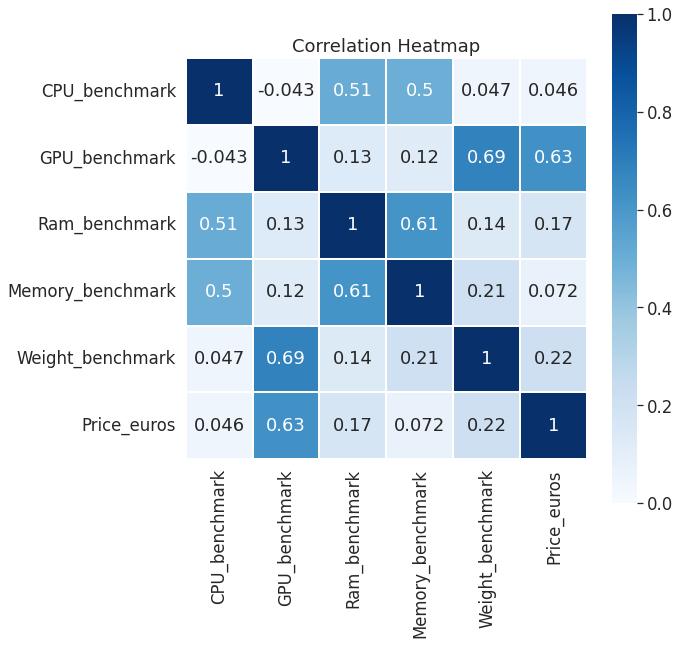
\includegraphics[scale=0.4]{Graphics/4520 final/Heat_map.png}
	\end{center}
	\caption{Architecture of our distributed certification service}
	\label{fig:heat}
\end{figure}

As shown above, the group started off with the correlation heat map. It can be seen that all factors selected are positively correlated with the price in euros, while the GPU benchmark has the most significant value of correlation. However, the CPU benchmark appears to have a minimal correlation value with the price, which the team did not expect. 

\section{PREDICTION MODEL TRAINING}

\subsection{LINEAR REGRESSION}

\subsubsection{MULTIPLE LINEAR REGRESSION}

The group first approach the data with linear regression. This method model the relationship between a scalar response Y and multiple explanatory variables $X_i$. In this case, benchmarking scores of CPU, GPU, RAM, memory, and weight are inputted as X. Price in euros is set to be Y. To ensure the regression result is fair, the group standardized all the X input before the data was input into the regression model. The default OLS regression model from the python library\cite{chen} is then been utilized, the result is shown in the figure below.

\begin{figure}[H]
	\begin{center}
		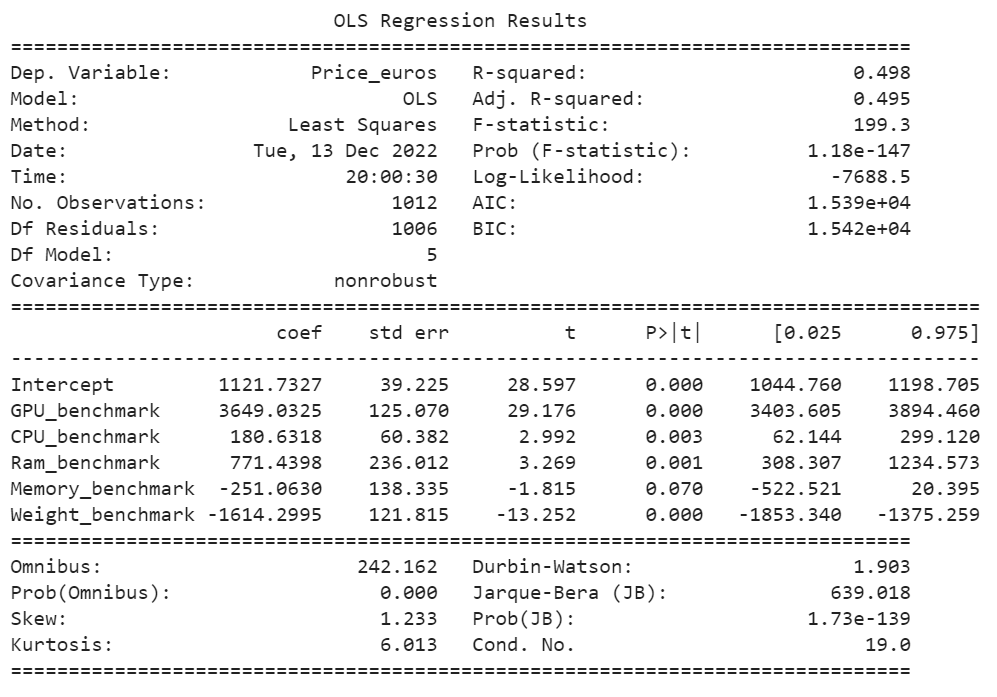
\includegraphics[scale=0.6]{Graphics/4520 final/OLS_regression.png}
	\end{center}
	\caption{Multiple linear regression results using OLS model}
	\label{fig:OLS}
\end{figure}

\noindent As shown in Figure~\ref{fig:OLS}, the overall R-squared value is around 0.498 (first row second column), which is considered to be acceptable. Among all the coefficient results, the team discovered that the GPU has the highest value (second row in "coef"), which conforms to the heatmap minimum result generated earlier. 

\subsubsection{SINGLE LINEAR REGRESSION}

To better understand how GPU would affect the price, the group then classified the GPUs according to their manufacturer brands. In this case, the team splitted the whole data set into three major categories: Intel GPUs, Nvidia GPUs, and AMD GPUs. For each individual category, a single linear regression was modeled between laptop price (Y) and GPU benchmark (X). All results are shown in Figure~\ref{fig:SLR}. 

\begin{figure}[H]
     \centering
     \begin{subfigure}
         \centering
         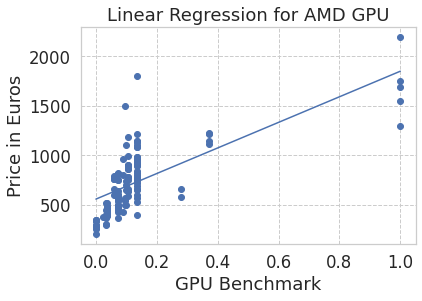
\includegraphics[scale=0.5]{Graphics/4520 final/AMD_GPU_LNR_0-1.png}
     \end{subfigure}
     \hfill
     \begin{subfigure}
         \centering
         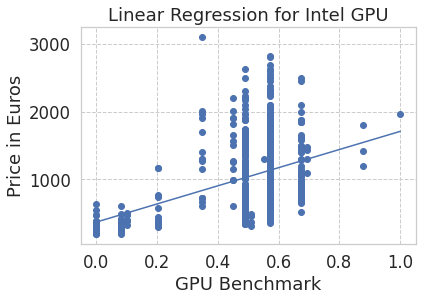
\includegraphics[scale=0.5]{Graphics/4520 final/Intel_GPU_LNR_0-1.png}
     \end{subfigure}
     \hfill
     \begin{subfigure}
         \centering
         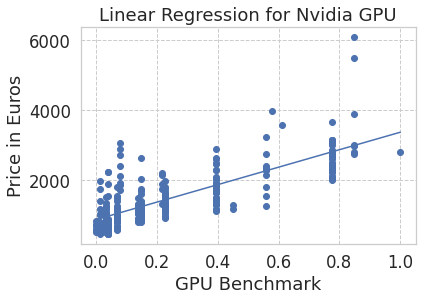
\includegraphics[scale=0.5]{Graphics/4520 final/Nvidia_GPU_LNR_0-1.png}
     \end{subfigure}
        \caption{Single linear regression results}
        \label{fig:SLR}
\end{figure}

\noindent Furthermore, the team calculated the R-squared value for each individual category to illustrate the effectiveness of the regression. The results were concluded in Table~\ref{tab:RSQR}. Among the three categories, Intel GPU has the lowest R-squared value. This is because Intel tends to have a lower price for newer GPU series, which may have higher benchmark scores. Therefore, the performance benchmarks for Intel GPUs may be unmatchable to their price.  As for AMD and Nvidia, their R-squared values are both above 0.5, therefore considered to be more positively related to their price relative to Intel GPUs. 

\begin{table}[h!]
\centering
\begin{tabular}{|c | c|} 
 \hline
 GPU Brand & R-Squared Value\\ [0.5ex] 
 \hline\hline
 AMD & 0.513 \\ 
 Intel & 0.513 \\ 
 Nvidia & 0.597 \\ [1ex] 
 \hline
\end{tabular}
\caption{Comparison of R-squared values for each GPU category.}
\label{tab:RSQR}
\end{table}

\subsubsection{LINEAR REGRESSION CROSS-VALIDATION}

To better examine the effectiveness of the linear regression model, the group chose the method of linear regression cross-validation. In this case, the data set was split randomly into 70\% of training data and 30\% of test data. The results are given in Table~\ref{tab:CRSV}. 

\begin{table}[h!]
\centering
\begin{tabular}{|c | c | c|} 
 \hline
Data Set & R-Squared Value for Training Data (70\%) & R-Squared Value for Testing Data (30\%)\\ [0.5ex] 
 \hline\hline
 All GPU & 0.446 & 0.294 \\ 
 AMD GPU & 0.550 & 0.463 \\
 Intel GPU & 0.161 & 0.138 \\ 
 Nvidia GPU & 0.609 & 0.589 \\ [1ex] 
 \hline
\end{tabular}
\caption{Cross-validation for each GPU category.}
\label{tab:CRSV}
\end{table}

\noindent The test dataset for each element generally would have a smaller R-Squared value compared to the training data. However, the test data R-squared value for all GPUs is particularly small (less than 70\% of the training data). This suggests that the similar issue described before in the previous section, that Intel GPUs may have unmatchable prices to benchmark scores. For this reason, all-GPU data is expected to be much more dispersive, resulting in a low R-squared value. 


%%%%%%%% Neural Network Overall %%%%%%%%%

\subsection{NEURAL NETWORK}

\begin{figure}[H]
	\begin{center}
		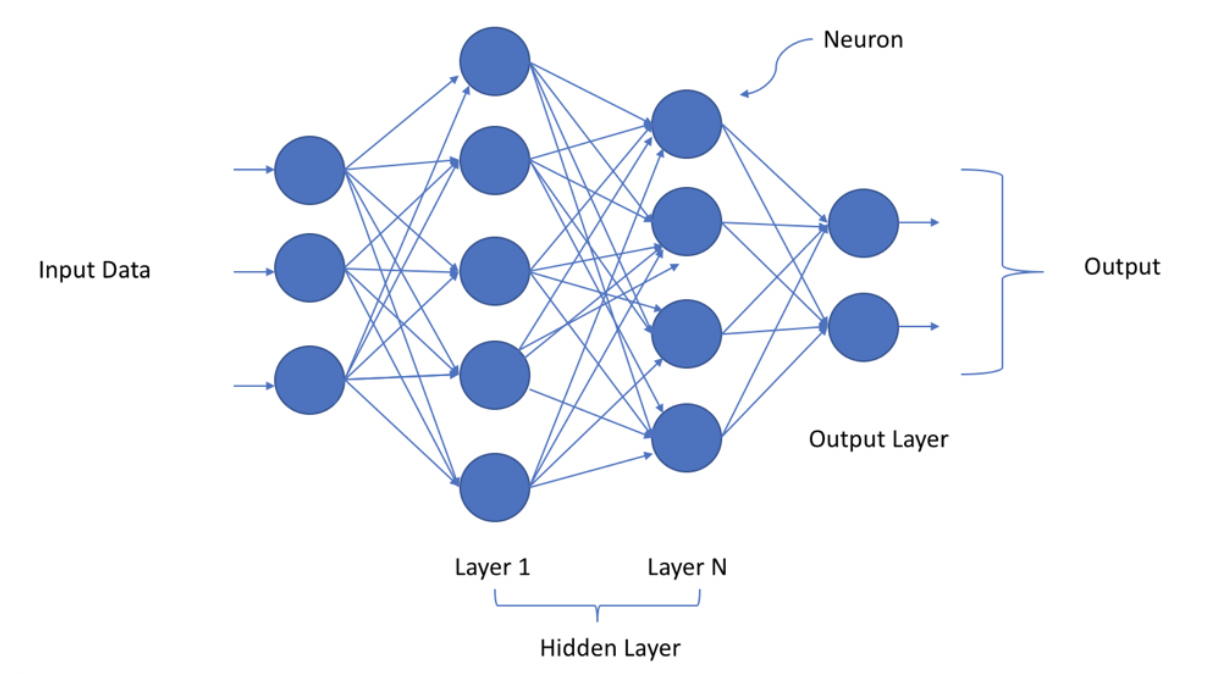
\includegraphics[scale=0.3]{Graphics/Neural Network Images/NN1.png}
	\end{center}
	\caption{Neural Network}
	\label{fig:NN1}
\end{figure}

\noindent In deep learning, a neural network is an artificial neural network made up of synthetic neurons or nodes, which is the analogy with biological neurons. The group used a neural network containing 1 input layer, 2 hidden layers, and 1 output layer. Different parameters were used for the neural network. For the input layer, 50 neurons were set. For the hidden layer, 25 neurons were set. As for the output layer, only one neuron was set because the team just needs one dependent variable - the price of the laptop. 
Within the model whose features were "GPU\_benchmark", "Memory\_benchmark", "CPU\_benchmark", "Weight\_benchmark", and "Ram\_benchmark", the neurons first took 50 numeric inputs. Then the team multiplied each one of the numeric units, including a weight which means how important each input is and plus a bias. The parameters of the neural network were shown in Table~\ref{tab:params_table}. As shown, there are 1431 parameters in total. \\

\begin{table}[ht]
    \centering
    \begin{tabular}{lllll}
\cline{1-3}
Layer  (type)      & Output Shape & Param \# &  &  \\ \cline{1-3}
dense\_16 (Dense)  & (None,  50)  & 300      &  &  \\
dense\_17 (Dense)  & (None,  20)  & 1020     &  &  \\
dense\_18 (Dense)  & (None,  5)   & 105      &  &  \\
dense\_19 (Dense)  & (None,  1)   & 6        &  &  \\ \cline{1-3}
\begin{tabular}[c]{@{}l@{}}Total params: 1,431\\ Trainable params: 1,431\\ Non-trainable params: 0\end{tabular} &              &          &  &  \\ \cline{1-3}
\end{tabular}
    \caption{Parameters of Neural Network \texttt{localhost}.}
    \label{tab:params_table}
\end{table}

\noindent To start with, the data was split into training data and testing data with the proportion of 7:3, 8:2, and 9:1. In these settings, the team then standardized each feature of the data using the following code shown in the following list. 

\begin{lstlisting}[language=Python, caption= Testing-Training Data splitting and Standardization,basicstyle=\tiny,captionpos=b]

X_raw, X_raw_test, Y, Y_test = train_test_split(data[features].values, data[label].values, test_size=0.1, random_state=42)

scaler = StandardSca aler()
scaler.fit(X_raw)
X = scaler.transform(X_raw)
X_test = scaler.transform(X_raw_test)

Y = Y.reshape((-1, 1))
Y_test = Y_test.reshape((-1, 1))

\end{lstlisting}


\newpage

\noindent In order to illustrate the data distribution, the team plotted the standardized result as shown in Figure~\ref{fig:NN4}. 

\begin{figure}[H]
	\begin{center}
		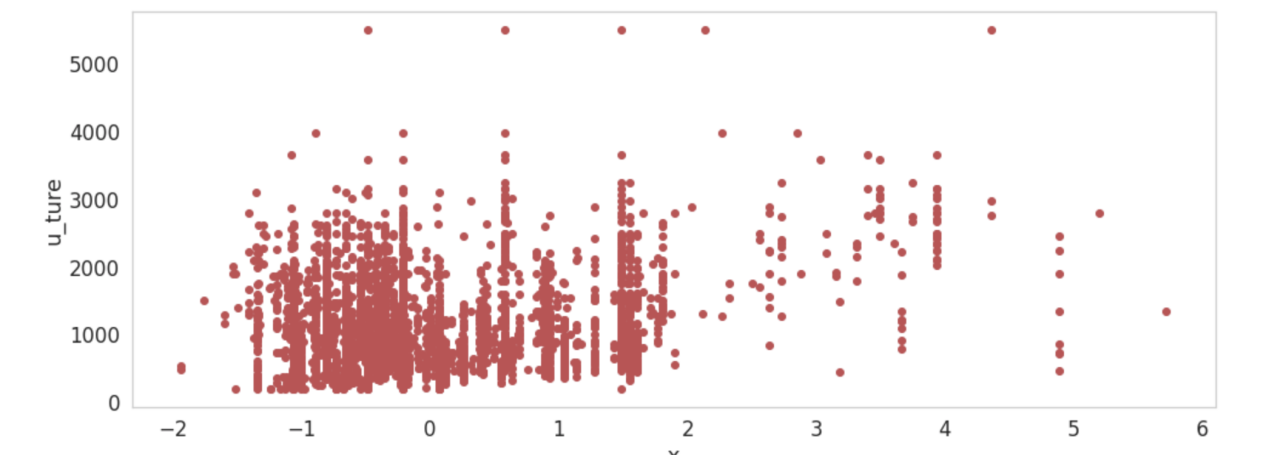
\includegraphics[scale=1.0]{Graphics/Neural Network Images/NN4.png}
	\end{center}
	\caption{Standardized Data}
	\label{fig:NN4}
\end{figure}


\noindent For the input layer and the hidden layer, the team used the “relu” function, which can be defined as:

\[f(x) = \left\{\begin{matrix}
0 \;\;for \;\;\;x<0\\ 
x \;\;for \;\;\;x\geqslant 0
\end{matrix}\right.\]

\noindent For the output, the team used the “linear” function, which can be defined as: 

\[f(x) = x\]

\noindent For the loss function’s metric, the team used the Mean Squared Error (MSE), which can be defined as:

\[\mathrm{MSE}=\frac{1}{n} \Sigma_{i=1}^n\left(y_i-\hat{y}_i\right)^2\]

\noindent Within this framework, the team used the following code to train the model:

\begin{lstlisting}[language=Python, caption= Code for training overall data, basicstyle=\tiny,captionpos=b]

    model=Sequential([
        Dense(units=50,kernel_initializer='normal',activation='relu'),    
        Dense(units=20,kernel_initializer='normal',activation='relu'),
        Dense(units=5,kernel_initializer='normal',activation='relu'),
        Dense(units=1,kernel_initializer='normal',activation='linear'),
    ])

    model.compile(
        optimizer=Adam(learning_rate=0.01),
        loss="mse",
        metrics=["mse"])

    history = model.fit(
        x=X,
        y=Y,
        batch_size=32,
        epochs=20,
        validation_data=(X_test, Y_test),
        verbose=1,
        shuffle=True,
    )

\end{lstlisting}

\noindent When the proportion of training data to testing data is 7:3, after 20 epochs, the MSEs of training data and testing data both converged. The resulting R-squared value, in this case, is 0.5400939, using the method shown in the following list. A snapshot of the output comparison is shown in Figure~\ref{fig:NN7-8}. An MSE plot is shown in Figure~\ref{fig:net}. \\

\begin{lstlisting}[language=Python, caption= R-Squared output code, basicstyle=\tiny,captionpos=b]
r2 = np.power(yhat - np.mean(Y_test), 2).sum() / np.power(Y_test - np.mean(Y_test), 2).sum()
r2

\end{lstlisting}

\begin{figure}[H]
         \centering
         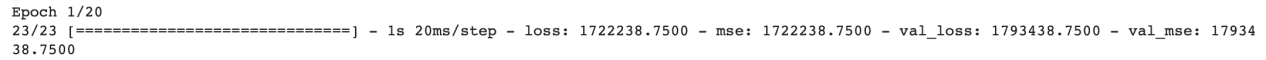
\includegraphics[width=\textwidth]{Graphics/Neural Network Images/NN7.png}
\end{figure}
     
\begin{figure}[H]
         \centering
         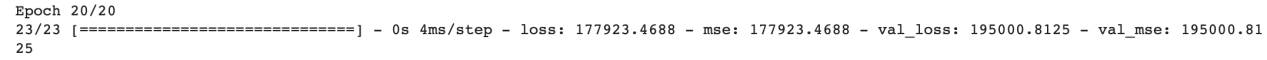
\includegraphics[width=\textwidth]{Graphics/Neural Network Images/NN8.png}
         \caption{Neural network output snapshot for overall data}
         \label{fig:NN7-8}
\end{figure}


\begin{figure}[H]
	\begin{center}
		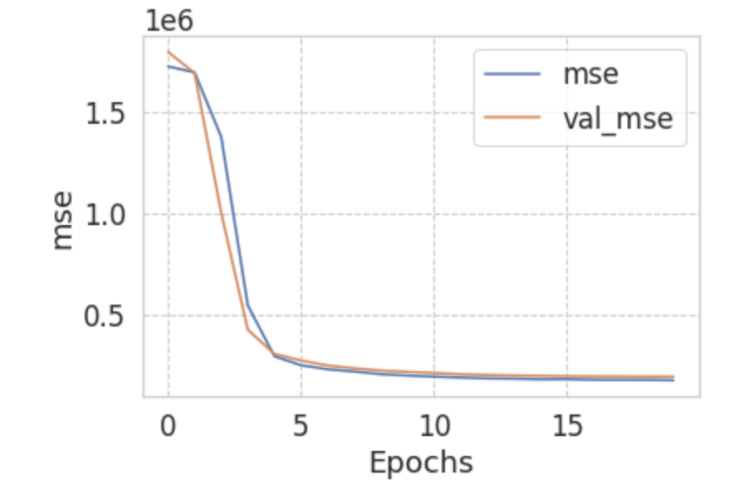
\includegraphics[scale=1.0]{Graphics/Neural Network Images/NN6.png}
	\end{center}
	\caption{MSE plot for overall data}
	\label{fig:net}
\end{figure}

\noindent As shown, the outcome above shows that the MSE for the training data changed from 1722238.75 in epoch 1 to 177923.4688 in epoch 20. And the MSE for the testing data changed from 1793438.75 in epoch 1 to 195000.8125 in epoch 20. The $R^2$ of the model is 0.54.\\





%%%%%%%% Neural Network Nvidia %%%%%%%%%


\noindent For the next step, the team changed the features of the data to “GPU\_benchmark” only to make the comparison with the linear regression method. The data set was divided into three categories according to the brands: Nvidia, AMD, and Intel. \\

\noindent The team started off this step with data only from Nvidia. The method used to train the data remained exactly the same, except for the “features” and the number of inputs. The code is shown in the following list. \\

\begin{lstlisting}[language=Python, caption= Code for training Nvidia data, basicstyle=\tiny,captionpos=b]
features_GPU_NV = [ "GPU_benchmark",]
label = "Price_euros"
model_GPU_NV=Sequential([
    Dense(units=25,kernel_initializer='normal',activation='relu'),
    Dense(units=15,kernel_initializer='normal',activation='relu'),
    Dense(units=5,kernel_initializer='normal',activation='relu'),
    Dense(units=1,kernel_initializer='normal',activation='linear'),
])

\end{lstlisting}


\noindent The resulting R-squared value, in this case, was calculated similarly using the method similar to the previous step, which is shown in the following list. A snapshot of the output comparison is shown in Figure~\ref{fig:NN12-13}. An MSE plot is shown in Figure 9. \\

\begin{lstlisting}[language=Python, caption= Code output for MSE Nvidia training, basicstyle=\tiny,captionpos=b]
r2_GPU_NV = np.power(yhat_GPU_NV - np.mean(Y_test_GPU_NV), 2).sum() / np.power(Y_test_GPU_NV - np.mean(Y_test_GPU_NV), 2).sum()
r2_GPU_NV
    
\end{lstlisting}


\begin{figure}[H]
         \centering
         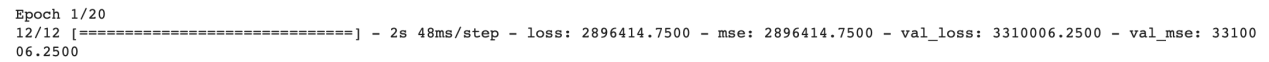
\includegraphics[width=\textwidth]{Graphics/Neural Network Images/NN12.png}
\end{figure}
     
\begin{figure}[H]
         \centering
         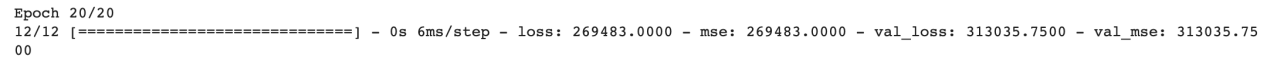
\includegraphics[width=\textwidth]{Graphics/Neural Network Images/NN13.png}
         \caption{Neural network output snapshot for Nvidia data}
         \label{fig:NN12-13}
\end{figure}

\begin{figure}[H]
	\begin{center}
		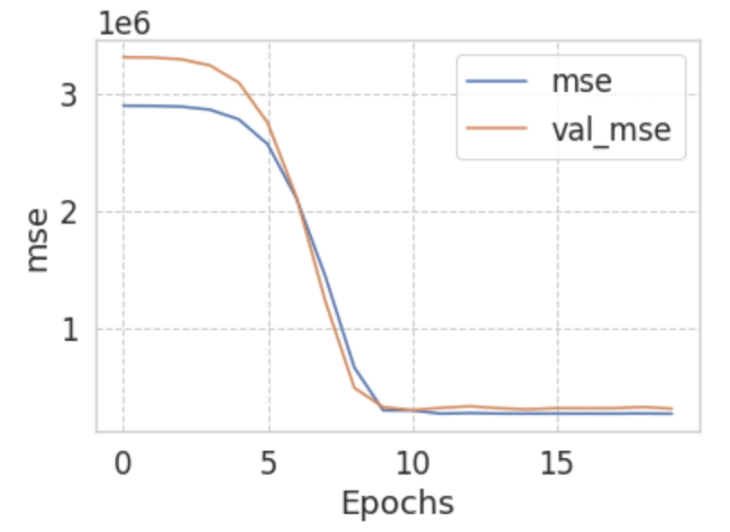
\includegraphics[scale=1.0]{Graphics/Neural Network Images/NN11.png}
    \caption{MSE plot for Nvidia data}
	\end{center}
	\label{fig:net2}
\end{figure}

\noindent As shown, the outcome above shows that the MSE for the training data changed from 2895840.2500 in epoch 1 to 271110.7188 in epoch 20. And the MSE for the test data changed from 3307747 in epoch 1 to 316232.0938 in epoch 20. The $R^2$ of the model is $0.36932928$.\\




%%%%%%%% Neural Network AMD %%%%%%%%%

\noindent Then, the group repeated similar steps for the AMD laptops. The training code is shown in the following list. 

\begin{lstlisting}[language=Python, caption= Code for training AMD data, basicstyle=\tiny,captionpos=b]
features_GPU_AMD = [ "GPU_benchmark",]
label = "Price_euros"
model_GPU_AMD=Sequential([
    Dense(units=25,kernel_initializer='normal',activation='relu'),
    Dense(units=10,kernel_initializer='normal',activation='relu'),
    Dense(units=5,kernel_initializer='normal',activation='relu'),
    Dense(units=1,kernel_initializer='normal',activation='linear'),
])
\end{lstlisting}

\noindent The resulting R-squared value, in this case, was calculated similarly using the method similar to the previous step, which is shown in the following list. A snapshot of the output comparison is shown in Figure~\ref{fig:NN18-19}. An MSE plot is shown in Figure~\ref{fig:NN17}. \\

\begin{lstlisting}[language=Python, caption= Code output for MSE AMD training,basicstyle=\tiny,captionpos=b]
r2_GPU_AMD = np.power(yhat_GPU_AMD - np.mean(Y_test_GPU_AMD), 2).sum() / np.power(Y_test_GPU_AMD - np.mean(Y_test_GPU_AMD), 2).sum()
r2_GPU_AMD

\end{lstlisting}

\newpage

\begin{figure}[H]
         \centering
         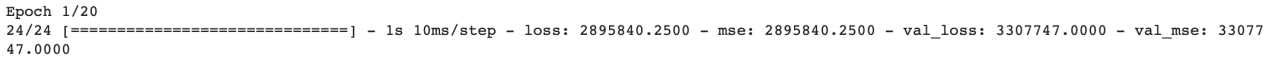
\includegraphics[width=\textwidth]{Graphics/Neural Network Images/NN18.png}
\end{figure}
     
\begin{figure}[H]
         \centering
         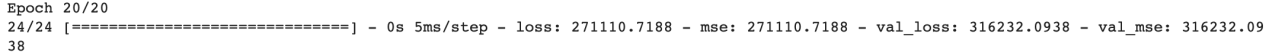
\includegraphics[width=\textwidth]{Graphics/Neural Network Images/NN19.png}
         \caption{Neural network output snapshot for AMD data}
         \label{fig:NN18-19}
\end{figure}


\begin{figure}[H]
	\begin{center}
		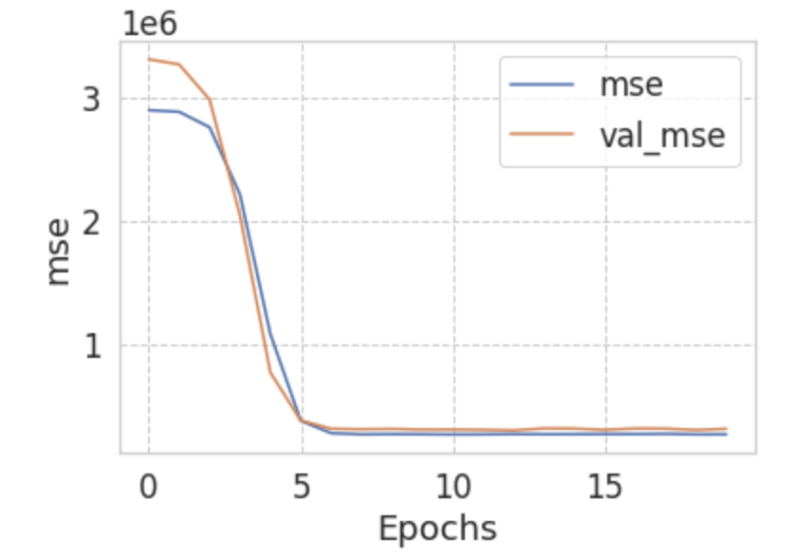
\includegraphics[scale=1.0]{Graphics/Neural Network Images/NN17.png}
	\end{center}
	\caption{MSE plot for AMD data}
	\label{fig:NN17}
\end{figure}

\noindent The outcome above shows that the MSE for the training data changed from 2895840.2500 in epoch 1 to 271110.7188 in epoch 20. And the MSE for the test data changed from 3307747 in epoch 1 to 316232.0938 in epoch 20. The $R^2$ of the model is 0.36932928. \\







%%%%%%%% Neural Network Intel %%%%%%%%%

\noindent Lastly, similar steps was repeated for the Intel laptop. The training code is shown in the following list. 

\begin{lstlisting}[language=Python, caption= Code for training Intel data, basicstyle=\tiny,captionpos=b]
features_GPU_Intel = [ "GPU_benchmark",]
label = "Price_euros"
model_GPU_Intel=Sequential([
    Dense(units=15,kernel_initializer='normal',activation='relu'),
    Dense(units=8,kernel_initializer='normal',activation='relu'),
    Dense(units=3,kernel_initializer='normal',activation='relu'),
    Dense(units=1,kernel_initializer='normal',activation='linear'),
])
\end{lstlisting}

\noindent The resulting R-squared value, in this case, was calculated similarly using the method similar to the previous step, which is shown in the following list. A snapshot of the output comparison is shown in Figure~\ref{fig:NN24-25}. An MSE plot is shown in Figure~\ref{fig:NN23}. \\

\begin{lstlisting}[language=Python, caption= Code output for MSE Intel training,basicstyle=\tiny,captionpos=b]
r2_GPU_Intel = np.power(yhat_GPU_Intel - np.mean(Y_test_GPU_Intel), 2).sum() / np.power(Y_test_GPU_Intel - np.mean(Y_test_GPU_Intel), 2).sum()
r2_GPU_Intel

\end{lstlisting}

\begin{figure}[H]
         \centering
         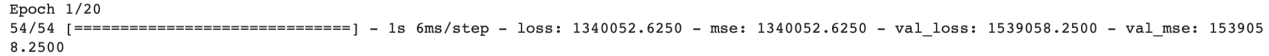
\includegraphics[width=\textwidth]{Graphics/Neural Network Images/NN24.png}
\end{figure}
     
\begin{figure}[H]
         \centering
         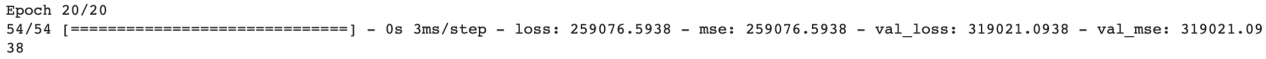
\includegraphics[width=\textwidth]{Graphics/Neural Network Images/NN25.png}
         \caption{Neural network output snapshot for Intel data}
         \label{fig:NN24-25}
\end{figure}


\begin{figure}[H]
	\begin{center}
		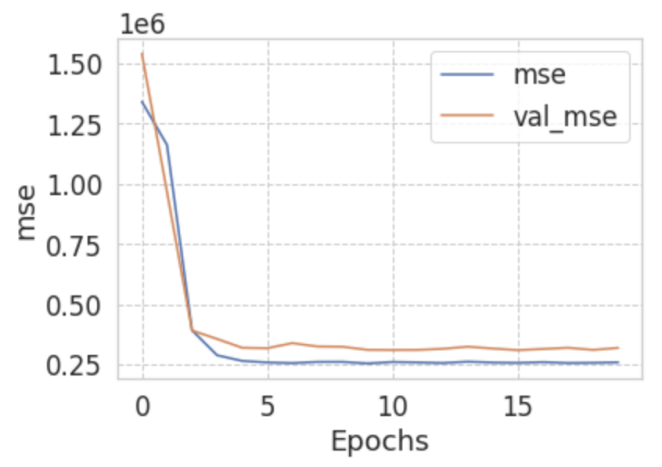
\includegraphics[scale=1.0]{Graphics/Neural Network Images/NN23.png}
	\end{center}
	\caption{MSE plot for Intel data}
	\label{fig:NN23}
\end{figure}

\noindent The outcome above shows that the MSE for the training data changed from 1340052.6250 in epoch 1 to 259076.5938 in epoch 20. And the MSE for the test data changed from 1539058.2500 in epoch 1 to 319021.0938 in epoch 20. The $R^2$ of the model is 0.168142. \\





%%%%%%%% Neural Network Conclusion %%%%%%%%%

\begin{table}[ht]
\centering
\begin{tabular}{lllll}
\cline{1-4}
\multicolumn{1}{|l|}{Data Set} & \multicolumn{1}{l|}{\begin{tabular}[c]{@{}l@{}}$R^2$ for test data\\ (train:test = 7:3)\end{tabular}} & \multicolumn{1}{l|}{\begin{tabular}[c]{@{}l@{}}$R^2$ for test data\\ (train:test = 8:2)\end{tabular}} & \multicolumn{1}{l|}{\begin{tabular}[c]{@{}l@{}}$R^2$ for test data\\ (train:test = 9:1)\end{tabular}} &  \\ \cline{1-4}
\multicolumn{1}{|l|}{All GPU}  & \multicolumn{1}{l|}{0.388}                                                                         & \multicolumn{1}{l|}{0.436}                                                                         & \multicolumn{1}{l|}{0.483}                                                                         &  \\ \cline{1-4}
\multicolumn{1}{|l|}{NVIDIA}   & \multicolumn{1}{l|}{0.362}                                                                         & \multicolumn{1}{l|}{0.404}                                                                         & \multicolumn{1}{l|}{0.442}                                                                         &  \\ \cline{1-4}
\multicolumn{1}{|l|}{AMD}      & \multicolumn{1}{l|}{0.366}                                                                         & \multicolumn{1}{l|}{0.412}                                                                         & \multicolumn{1}{l|}{0.464}                                                                         &  \\ \cline{1-4}
\multicolumn{1}{|l|}{INTEL}    & \multicolumn{1}{l|}{0.165}                                                                         & \multicolumn{1}{l|}{0.156}                                                                         & \multicolumn{1}{l|}{0.157}                                                                         &  \\ \cline{1-4}

\end{tabular}
    \caption{ Results\texttt{localhost}.}
    \label{tab:results_table}
\end{table}


\noindent To sum up, the team compared four sets of results in Table~\ref{tab:results_table}. Presumably due to the limited amount of data, the neural network model used in this project is not accurate enough compared to the linear regression method. As the team members kept increasing the ratio of training data to test data, the $R^2$ of the model increased. This implies that the more data involved in training the model, the better the model performs. A potential improving method can be considered a data set with a larger data quantity and training the model more precisely.\\




\section{CONCLUSION}




By collecting several parameters, adding several benchmarks as the new inputs, and this paper constructs a laptop price prediction model. The main work is as follows:\\

\subsection{DATA COLLECTION}
To better quantify the relationship between the five parameters chosen and the laptop price, the team substituted the score of each laptop component’s theoretical performance to the original model names, namely the benchmark. Doing so can give the potential customers a more precise metric to estimate if the price of the laptops and their components is set appropriately.\\
\subsection{LINEAR REGRESSION}
Using python as our programming language, After modeling, the $R^2$ of using all six parameters equal to 0.498. Due to the $R^2$ 's shortcomings, the team chose the GPU benchmark as our only independent variable to build the model, the coefficient of which is much higher than other parameters. As the $R^2$ of which is also not ideal, the team divided GPUs into 3 brands. As a result, AMD GPUs have significantly superior $R^2$ ratings than Intel GPUs. The group assumes this is because Intel's GPU performance in this dataset does not correspond to its price. Then the team randomly chose 70\% of the data set as the training data, the rest as test data, as the cross-validation method. All of the $R^2$ values for the test data are lower than but near to those for the corresponding training data, suggesting that these models are feasible.\\
\subsection{NEURAL NETWORK REGRESSION}
The second method used was neural network regression. Based on the experience, the team set 2 hidden layers. Mean square error was used as their metric. The MSE of training data and test data were relatively close. Additionally, the neural network's three GPU $R^2$s are all lower than those of linear regression, which goes somewhat against conventional wisdom. As a result, the team increased their ratio of training data to test data from 7:3 to 8:2 to 9:1. It shows that the $R^2$ of AMD and Nvidia keep going up as there are more and more training data comes into play.\\






\section{FUTURE WORK}

In this project, the focus is primarily on helping customers who are relatively familiar with laptops, they are required to possess certain knowledge about the models of different computer components, or at least understand the basic components of laptops. In the future, more advice can be provided on how to pick the right laptop components totally depending on customers' preferences and budget, by doing so can the team reach a wider application field of different customers and decrease its constraints.\\


\noindent Besides, more data can be absorbed to improve the price prediction accuracy, since when discussing the result of different brands of GPUs, the team experienced data inaccuracy due to the shortage of numbers of data on Intel GPUs. The team will also consider broadening the topic from laptops to PCs.\\


\newpage
\singlespacing
\bibliographystyle{IEEEtran}
\bibliography{references}


%------ To create Appendix with additional stuff -------%
\newpage
\appendix
\section{APPENDIX}

\href{https://github.com/zw2788/MECE4520\_project/blob/main/MECE\_4520\_LaptopPrediction/Method\_Linear.ipynb}{Code for linear regression (train: test= 7:3)}.\\


%Code for linear regression (train: test= 7:3):\\

%\text{https://github.com/zw2788/MECE4520\_project/blob/main/MECE\_4520\_LaptopPrediction/Method\_Linear.ipynb}\\
\noindent
\href{https://github.com/zw2788/MECE4520\_project/blob/main/MECE\_4520\_LaptopPrediction/test\_0.3.ipynb}{Code for Neural Network (train: test= 7:3)}.\\

\noindent
\href{https://github.com/zw2788/MECE4520\_project/blob/main/MECE\_4520\_LaptopPrediction/test_0.2.ipynb}{Code for Neural Network (train: test= 8:2)}.\\

\noindent
\href{https://github.com/zw2788/MECE4520\_project/blob/main/MECE\_4520\_LaptopPrediction/test\_0.1.ipynb}{Code for Neural Network (train: test= 9:1)}.\\

\noindent
\href{https://github.com/noct-A/Laptop-Price-Prediction-MECE4520-Project-Report}{Laptop Price Prediction Report LaTex}

\begin{lstlisting}[language=Python,  basicstyle=\tiny,]


\end{lstlisting}

\end{document}
